\documentclass[]{article}
\usepackage{lmodern}
\usepackage{amssymb,amsmath}
\usepackage{ifxetex,ifluatex}
\usepackage{fixltx2e} % provides \textsubscript
\ifnum 0\ifxetex 1\fi\ifluatex 1\fi=0 % if pdftex
  \usepackage[T1]{fontenc}
  \usepackage[utf8]{inputenc}
\else % if luatex or xelatex
  \ifxetex
    \usepackage{mathspec}
  \else
    \usepackage{fontspec}
  \fi
  \defaultfontfeatures{Ligatures=TeX,Scale=MatchLowercase}
\fi
% use upquote if available, for straight quotes in verbatim environments
\IfFileExists{upquote.sty}{\usepackage{upquote}}{}
% use microtype if available
\IfFileExists{microtype.sty}{%
\usepackage{microtype}
\UseMicrotypeSet[protrusion]{basicmath} % disable protrusion for tt fonts
}{}
\usepackage[margin=1in]{geometry}
\usepackage{hyperref}
\hypersetup{unicode=true,
            pdftitle={Milestone 2},
            pdfauthor={Anh Le, Eve Wicksteed},
            pdfborder={0 0 0},
            breaklinks=true}
\urlstyle{same}  % don't use monospace font for urls
\usepackage{color}
\usepackage{fancyvrb}
\newcommand{\VerbBar}{|}
\newcommand{\VERB}{\Verb[commandchars=\\\{\}]}
\DefineVerbatimEnvironment{Highlighting}{Verbatim}{commandchars=\\\{\}}
% Add ',fontsize=\small' for more characters per line
\usepackage{framed}
\definecolor{shadecolor}{RGB}{248,248,248}
\newenvironment{Shaded}{\begin{snugshade}}{\end{snugshade}}
\newcommand{\AlertTok}[1]{\textcolor[rgb]{0.94,0.16,0.16}{#1}}
\newcommand{\AnnotationTok}[1]{\textcolor[rgb]{0.56,0.35,0.01}{\textbf{\textit{#1}}}}
\newcommand{\AttributeTok}[1]{\textcolor[rgb]{0.77,0.63,0.00}{#1}}
\newcommand{\BaseNTok}[1]{\textcolor[rgb]{0.00,0.00,0.81}{#1}}
\newcommand{\BuiltInTok}[1]{#1}
\newcommand{\CharTok}[1]{\textcolor[rgb]{0.31,0.60,0.02}{#1}}
\newcommand{\CommentTok}[1]{\textcolor[rgb]{0.56,0.35,0.01}{\textit{#1}}}
\newcommand{\CommentVarTok}[1]{\textcolor[rgb]{0.56,0.35,0.01}{\textbf{\textit{#1}}}}
\newcommand{\ConstantTok}[1]{\textcolor[rgb]{0.00,0.00,0.00}{#1}}
\newcommand{\ControlFlowTok}[1]{\textcolor[rgb]{0.13,0.29,0.53}{\textbf{#1}}}
\newcommand{\DataTypeTok}[1]{\textcolor[rgb]{0.13,0.29,0.53}{#1}}
\newcommand{\DecValTok}[1]{\textcolor[rgb]{0.00,0.00,0.81}{#1}}
\newcommand{\DocumentationTok}[1]{\textcolor[rgb]{0.56,0.35,0.01}{\textbf{\textit{#1}}}}
\newcommand{\ErrorTok}[1]{\textcolor[rgb]{0.64,0.00,0.00}{\textbf{#1}}}
\newcommand{\ExtensionTok}[1]{#1}
\newcommand{\FloatTok}[1]{\textcolor[rgb]{0.00,0.00,0.81}{#1}}
\newcommand{\FunctionTok}[1]{\textcolor[rgb]{0.00,0.00,0.00}{#1}}
\newcommand{\ImportTok}[1]{#1}
\newcommand{\InformationTok}[1]{\textcolor[rgb]{0.56,0.35,0.01}{\textbf{\textit{#1}}}}
\newcommand{\KeywordTok}[1]{\textcolor[rgb]{0.13,0.29,0.53}{\textbf{#1}}}
\newcommand{\NormalTok}[1]{#1}
\newcommand{\OperatorTok}[1]{\textcolor[rgb]{0.81,0.36,0.00}{\textbf{#1}}}
\newcommand{\OtherTok}[1]{\textcolor[rgb]{0.56,0.35,0.01}{#1}}
\newcommand{\PreprocessorTok}[1]{\textcolor[rgb]{0.56,0.35,0.01}{\textit{#1}}}
\newcommand{\RegionMarkerTok}[1]{#1}
\newcommand{\SpecialCharTok}[1]{\textcolor[rgb]{0.00,0.00,0.00}{#1}}
\newcommand{\SpecialStringTok}[1]{\textcolor[rgb]{0.31,0.60,0.02}{#1}}
\newcommand{\StringTok}[1]{\textcolor[rgb]{0.31,0.60,0.02}{#1}}
\newcommand{\VariableTok}[1]{\textcolor[rgb]{0.00,0.00,0.00}{#1}}
\newcommand{\VerbatimStringTok}[1]{\textcolor[rgb]{0.31,0.60,0.02}{#1}}
\newcommand{\WarningTok}[1]{\textcolor[rgb]{0.56,0.35,0.01}{\textbf{\textit{#1}}}}
\usepackage{longtable,booktabs}
\usepackage{graphicx,grffile}
\makeatletter
\def\maxwidth{\ifdim\Gin@nat@width>\linewidth\linewidth\else\Gin@nat@width\fi}
\def\maxheight{\ifdim\Gin@nat@height>\textheight\textheight\else\Gin@nat@height\fi}
\makeatother
% Scale images if necessary, so that they will not overflow the page
% margins by default, and it is still possible to overwrite the defaults
% using explicit options in \includegraphics[width, height, ...]{}
\setkeys{Gin}{width=\maxwidth,height=\maxheight,keepaspectratio}
\IfFileExists{parskip.sty}{%
\usepackage{parskip}
}{% else
\setlength{\parindent}{0pt}
\setlength{\parskip}{6pt plus 2pt minus 1pt}
}
\setlength{\emergencystretch}{3em}  % prevent overfull lines
\providecommand{\tightlist}{%
  \setlength{\itemsep}{0pt}\setlength{\parskip}{0pt}}
\setcounter{secnumdepth}{0}
% Redefines (sub)paragraphs to behave more like sections
\ifx\paragraph\undefined\else
\let\oldparagraph\paragraph
\renewcommand{\paragraph}[1]{\oldparagraph{#1}\mbox{}}
\fi
\ifx\subparagraph\undefined\else
\let\oldsubparagraph\subparagraph
\renewcommand{\subparagraph}[1]{\oldsubparagraph{#1}\mbox{}}
\fi

%%% Use protect on footnotes to avoid problems with footnotes in titles
\let\rmarkdownfootnote\footnote%
\def\footnote{\protect\rmarkdownfootnote}

%%% Change title format to be more compact
\usepackage{titling}

% Create subtitle command for use in maketitle
\providecommand{\subtitle}[1]{
  \posttitle{
    \begin{center}\large#1\end{center}
    }
}

\setlength{\droptitle}{-2em}

  \title{Milestone 2}
    \pretitle{\vspace{\droptitle}\centering\huge}
  \posttitle{\par}
    \author{Anh Le, Eve Wicksteed}
    \preauthor{\centering\large\emph}
  \postauthor{\par}
    \date{}
    \predate{}\postdate{}
  

\begin{document}
\maketitle

\hypertarget{air-quality-data}{%
\section{Air Quality Data}\label{air-quality-data}}

\hypertarget{introduction}{%
\subsection{Introduction}\label{introduction}}

The adverse affects of air pollution on health are well documented and
air pollution can lead to a large range of diseases and increased
morbidity and mortality (Younger et al., 2008). Adverse health impacts
include, but are not limited to, lung cancer risk, respiritory
infections, allergic disease and asthma (Younger et al., 2008; Shea et
al., 2008). These health risks can affect a large proportion of the
population as many different groups are vulnerable to the effects of air
pollution including infants, children, the elderly, people with impaired
immune systems, and people who work or are physically active outdoors
(Matooane et al., 2004).

Because of the many, and severe, impacts of air quality, it is important
to understand patterns in the data. We have a dataset of air quality
observations as well as temperature and humidity data which we will use
to gain understanding of the patterns and impacts of weather on air
quality.

\hypertarget{data-description}{%
\subsection{Data Description}\label{data-description}}

The air quality
\href{https://archive.ics.uci.edu/ml/datasets/Air+Quality}{dataset} used
in this analysis was obtained from the University of California Irvine
Machine learning Repository. It was contributed by Saverio De Vito from
the National Agency for New Technologies, Energy and Sustainable
Economic Development.

The dataset contains 15 variables and 9358 observations of hourly
averaged responses from an Air Quality Chemical Multisensor Device. Data
were recorded from March 2004 to February 2005, in a significantly
polluted area, at road level, within a city in Italy. Variables include
the date and time each response was recorded, and the corresponding
concentrations of 13 air pollutants analyzed by the sensor device.
Missing values are tagged with -200 value. Below is the entire variable
set:

\begin{longtable}[]{@{}lll@{}}
\toprule
Variables & Type & Description\tabularnewline
\midrule
\endhead
Date & character & Date (DD/MM/YYYY)\tabularnewline
Time & time & Time (HH.MM.SS)\tabularnewline
CO(GT) & double & True hourly averaged concentration CO in mg/m\^{}3
(reference analyzer)\tabularnewline
PT08.S1(CO) & integer & PT08.S1 (tin oxide) hourly averaged sensor
response (nominally CO targeted)\tabularnewline
NMHC(GT) & integer & True hourly averaged overall Non Metanic
HydroCarbons concentration in microg/m\^{}3 (reference
analyzer)\tabularnewline
C6H6(GT) & double & True hourly averaged Benzene concentration in
microg/m\^{}3 (reference analyzer)\tabularnewline
PT08.S2(NMHC) & integer & PT08.S2 (titania) hourly averaged sensor
response (nominally NMHC targeted)\tabularnewline
NOx(GT) & integer & True hourly averaged NOx concentration in ppb
(reference analyzer)\tabularnewline
PT08.S3(NOx) & integer & PT08.S3 (tungsten oxide) hourly averaged sensor
response (nominally NOx targeted)\tabularnewline
NO2(GT) & integer & True hourly averaged NO2 concentration in
microg/m\^{}3 (reference analyzer)\tabularnewline
PT08.S4(NO2) & integer & PT08.S4 (tungsten oxide) hourly averaged sensor
response (nominally NO2 targeted)\tabularnewline
PT08.S5(O3) & integer & PT08.S5 (indium oxide) hourly averaged sensor
response (nominally O3 targeted)\tabularnewline
T & double & Temperature in °C\tabularnewline
RH & double & Relative Humidity (\%)\tabularnewline
AH & double & AH Absolute Humidity\tabularnewline
\bottomrule
\end{longtable}

\hypertarget{exploring-the-dataset}{%
\subsection{Exploring the dataset}\label{exploring-the-dataset}}

\begin{Shaded}
\begin{Highlighting}[]
\CommentTok{# first we read the data in}
\NormalTok{airq <-}\StringTok{ }\NormalTok{readr}\OperatorTok{::}\KeywordTok{read_csv}\NormalTok{(here}\OperatorTok{::}\KeywordTok{here}\NormalTok{(}\StringTok{"data"}\NormalTok{,}\StringTok{"airquality.csv"}\NormalTok{))}
\end{Highlighting}
\end{Shaded}

\begin{verbatim}
## Parsed with column specification:
## cols(
##   Date = col_date(format = ""),
##   Time = col_time(format = ""),
##   `CO(GT)` = col_double(),
##   `PT08.S1(CO)` = col_integer(),
##   `NMHC(GT)` = col_integer(),
##   `C6H6(GT)` = col_double(),
##   `PT08.S2(NMHC)` = col_integer(),
##   `NOx(GT)` = col_integer(),
##   `PT08.S3(NOx)` = col_integer(),
##   `NO2(GT)` = col_integer(),
##   `PT08.S4(NO2)` = col_integer(),
##   `PT08.S5(O3)` = col_integer(),
##   T = col_double(),
##   RH = col_double(),
##   AH = col_double()
## )
\end{verbatim}

\begin{Shaded}
\begin{Highlighting}[]
\NormalTok{DT}\OperatorTok{::}\KeywordTok{datatable}\NormalTok{(airq)}
\end{Highlighting}
\end{Shaded}

\includegraphics{milestone2_files/figure-latex/read data-1.pdf}

\hypertarget{summary-statistics}{%
\subsubsection{Summary Statistics}\label{summary-statistics}}

The following shows the five-number stats summary for each variable:

\begin{Shaded}
\begin{Highlighting}[]
\CommentTok{# Five-number summary for each variable}
\KeywordTok{summary}\NormalTok{(airq)}
\end{Highlighting}
\end{Shaded}

\begin{verbatim}
##       Date                Time              CO(GT)         PT08.S1(CO)  
##  Min.   :2004-03-10   Length:9357       Min.   :-200.00   Min.   :-200  
##  1st Qu.:2004-06-16   Class1:hms        1st Qu.:   0.60   1st Qu.: 921  
##  Median :2004-09-21   Class2:difftime   Median :   1.50   Median :1053  
##  Mean   :2004-09-21   Mode  :numeric    Mean   : -34.21   Mean   :1049  
##  3rd Qu.:2004-12-28                     3rd Qu.:   2.60   3rd Qu.:1221  
##  Max.   :2005-04-04                     Max.   :  11.90   Max.   :2040  
##     NMHC(GT)         C6H6(GT)        PT08.S2(NMHC)       NOx(GT)      
##  Min.   :-200.0   Min.   :-200.000   Min.   :-200.0   Min.   :-200.0  
##  1st Qu.:-200.0   1st Qu.:   4.000   1st Qu.: 711.0   1st Qu.:  50.0  
##  Median :-200.0   Median :   7.900   Median : 895.0   Median : 141.0  
##  Mean   :-159.1   Mean   :   1.866   Mean   : 894.6   Mean   : 168.6  
##  3rd Qu.:-200.0   3rd Qu.:  13.600   3rd Qu.:1105.0   3rd Qu.: 284.0  
##  Max.   :1189.0   Max.   :  63.700   Max.   :2214.0   Max.   :1479.0  
##   PT08.S3(NOx)     NO2(GT)         PT08.S4(NO2)   PT08.S5(O3)    
##  Min.   :-200   Min.   :-200.00   Min.   :-200   Min.   :-200.0  
##  1st Qu.: 637   1st Qu.:  53.00   1st Qu.:1185   1st Qu.: 700.0  
##  Median : 794   Median :  96.00   Median :1446   Median : 942.0  
##  Mean   : 795   Mean   :  58.15   Mean   :1391   Mean   : 975.1  
##  3rd Qu.: 960   3rd Qu.: 133.00   3rd Qu.:1662   3rd Qu.:1255.0  
##  Max.   :2683   Max.   : 340.00   Max.   :2775   Max.   :2523.0  
##        T                  RH                AH           
##  Min.   :-200.000   Min.   :-200.00   Min.   :-200.0000  
##  1st Qu.:  10.900   1st Qu.:  34.10   1st Qu.:   0.6923  
##  Median :  17.200   Median :  48.60   Median :   0.9768  
##  Mean   :   9.778   Mean   :  39.49   Mean   :  -6.8376  
##  3rd Qu.:  24.100   3rd Qu.:  61.90   3rd Qu.:   1.2962  
##  Max.   :  44.600   Max.   :  88.70   Max.   :   2.2310
\end{verbatim}

The following shows some preliminary info on the air quality dataset
that we are using. We record the number of total observations, number of
missing observations, percentage of missing values and the number of
usable observations.

\begin{Shaded}
\begin{Highlighting}[]
\CommentTok{# Look at missing values for each variable}
\NormalTok{missing =}\StringTok{ }\KeywordTok{list}\NormalTok{()}
\ControlFlowTok{for}\NormalTok{(i }\ControlFlowTok{in} \DecValTok{1}\OperatorTok{:}\DecValTok{15}\NormalTok{) \{}
\NormalTok{  l =}\StringTok{ }\KeywordTok{length}\NormalTok{(}\KeywordTok{which}\NormalTok{(airq[i] }\OperatorTok{==}\StringTok{ }\DecValTok{-200}\NormalTok{))}
\NormalTok{  missing[[i]] =}\StringTok{ }\NormalTok{l}
\NormalTok{\}}
\NormalTok{obs =}\StringTok{ }\KeywordTok{list}\NormalTok{()}
\ControlFlowTok{for}\NormalTok{(i }\ControlFlowTok{in} \DecValTok{1}\OperatorTok{:}\DecValTok{15}\NormalTok{) \{}
\NormalTok{  o =}\StringTok{ }\KeywordTok{length}\NormalTok{(airq[[i]])}
\NormalTok{  obs[[i]] =}\StringTok{ }\NormalTok{o}
\NormalTok{\}}
\NormalTok{dfmissing =}\StringTok{ }\KeywordTok{data.frame}\NormalTok{(Variables, }
                       \KeywordTok{matrix}\NormalTok{(}\KeywordTok{unlist}\NormalTok{(missing), }\DataTypeTok{nrow=}\KeywordTok{length}\NormalTok{(missing), }\DataTypeTok{byrow=}\NormalTok{T),}
                       \KeywordTok{matrix}\NormalTok{(}\KeywordTok{unlist}\NormalTok{(obs), }\DataTypeTok{nrow=}\KeywordTok{length}\NormalTok{(missing), }\DataTypeTok{byrow=}\NormalTok{T))}
\KeywordTok{names}\NormalTok{(dfmissing)[}\KeywordTok{names}\NormalTok{(dfmissing) }\OperatorTok{==}\StringTok{ "matrix.unlist.missing...nrow...length.missing...byrow...T."}\NormalTok{] =}\StringTok{ "Count of Missing Values"}
\KeywordTok{names}\NormalTok{(dfmissing)[}\KeywordTok{names}\NormalTok{(dfmissing) }\OperatorTok{==}\StringTok{ "matrix.unlist.obs...nrow...length.missing...byrow...T."}\NormalTok{] =}\StringTok{ "Total Observations"}
\NormalTok{dfmissing }\OperatorTok\StringTok{ }
\StringTok{  }\KeywordTok{mutate}\NormalTok{(}\StringTok{`}\DataTypeTok{% Missing Values}\StringTok{`}\NormalTok{ =}\StringTok{ `}\DataTypeTok{Count of Missing Values}\StringTok{`}\OperatorTok{/}\StringTok{`}\DataTypeTok{Total Observations}\StringTok{`}\OperatorTok{*}\DecValTok{100}\NormalTok{) }\OperatorTok
\StringTok{  }\KeywordTok{mutate}\NormalTok{(}\StringTok{`}\DataTypeTok{Usable Observations}\StringTok{`}\NormalTok{ =}\StringTok{ `}\DataTypeTok{Total Observations}\StringTok{`} \OperatorTok{-}\StringTok{ `}\DataTypeTok{Count of Missing Values}\StringTok{`}\NormalTok{)}
\end{Highlighting}
\end{Shaded}

\begin{verbatim}
##        Variables Count of Missing Values Total Observations
## 1           Date                       0               9357
## 2           Time                       0               9357
## 3         CO(GT)                    1683               9357
## 4    PT08.S1(CO)                     366               9357
## 5       NMHC(GT)                    8443               9357
## 6       C6H6(GT)                     366               9357
## 7  PT08.S2(NMHC)                     366               9357
## 8        NOx(GT)                    1639               9357
## 9   PT08.S3(NOx)                     366               9357
## 10       NO2(GT)                    1642               9357
## 11  PT08.S4(NO2)                     366               9357
## 12   PT08.S5(O3)                     366               9357
## 13             T                     366               9357
## 14            RH                     366               9357
## 15            AH                     366               9357
##    % Missing Values Usable Observations
## 1           0.00000                9357
## 2           0.00000                9357
## 3          17.98653                7674
## 4           3.91151                8991
## 5          90.23191                 914
## 6           3.91151                8991
## 7           3.91151                8991
## 8          17.51630                7718
## 9           3.91151                8991
## 10         17.54836                7715
## 11          3.91151                8991
## 12          3.91151                8991
## 13          3.91151                8991
## 14          3.91151                8991
## 15          3.91151                8991
\end{verbatim}

From this we see that for many of the observations less than 4\% of the
data is missing. This is adequate for the research we are conducting.

\hypertarget{graph-1-correlogram-of-pollutants}{%
\subsubsection{Graph 1: Correlogram of
pollutants}\label{graph-1-correlogram-of-pollutants}}

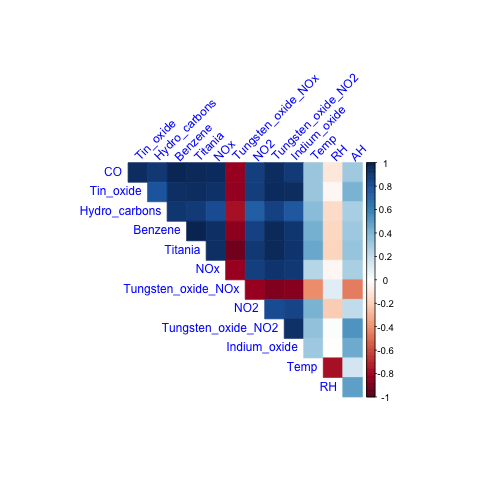
\includegraphics{../Images/correlation.png}

Looking at the correlations of the pollutants with weather, we can see
that for all pollutants except NOx, temperature (T) is positively
correlated, although weakly so. This means that higher temperatures
correspond to higher concentrations of the gases. Relative humidity (RH)
is negatively and correlated to temperature and has a weak negative
correlation to the concentrations of pollutants, except NOx. Absolute
humidity (AH) has stronger correlations, mostly positive, although, like
temperature, it has a negative correlation with NOx.

\hypertarget{graph-2-concentration-of-some-air-pollutants-temperature-humidity-over-time-daily-average}{%
\subsubsection{Graph 2: Concentration of some Air Pollutants,
Temperature, Humidity over Time, daily
average}\label{graph-2-concentration-of-some-air-pollutants-temperature-humidity-over-time-daily-average}}

The plot below shows the \textbf{daily} averaged concentrations of some
of the pollutants (tin oxide, benzene, and Titania) for a year.

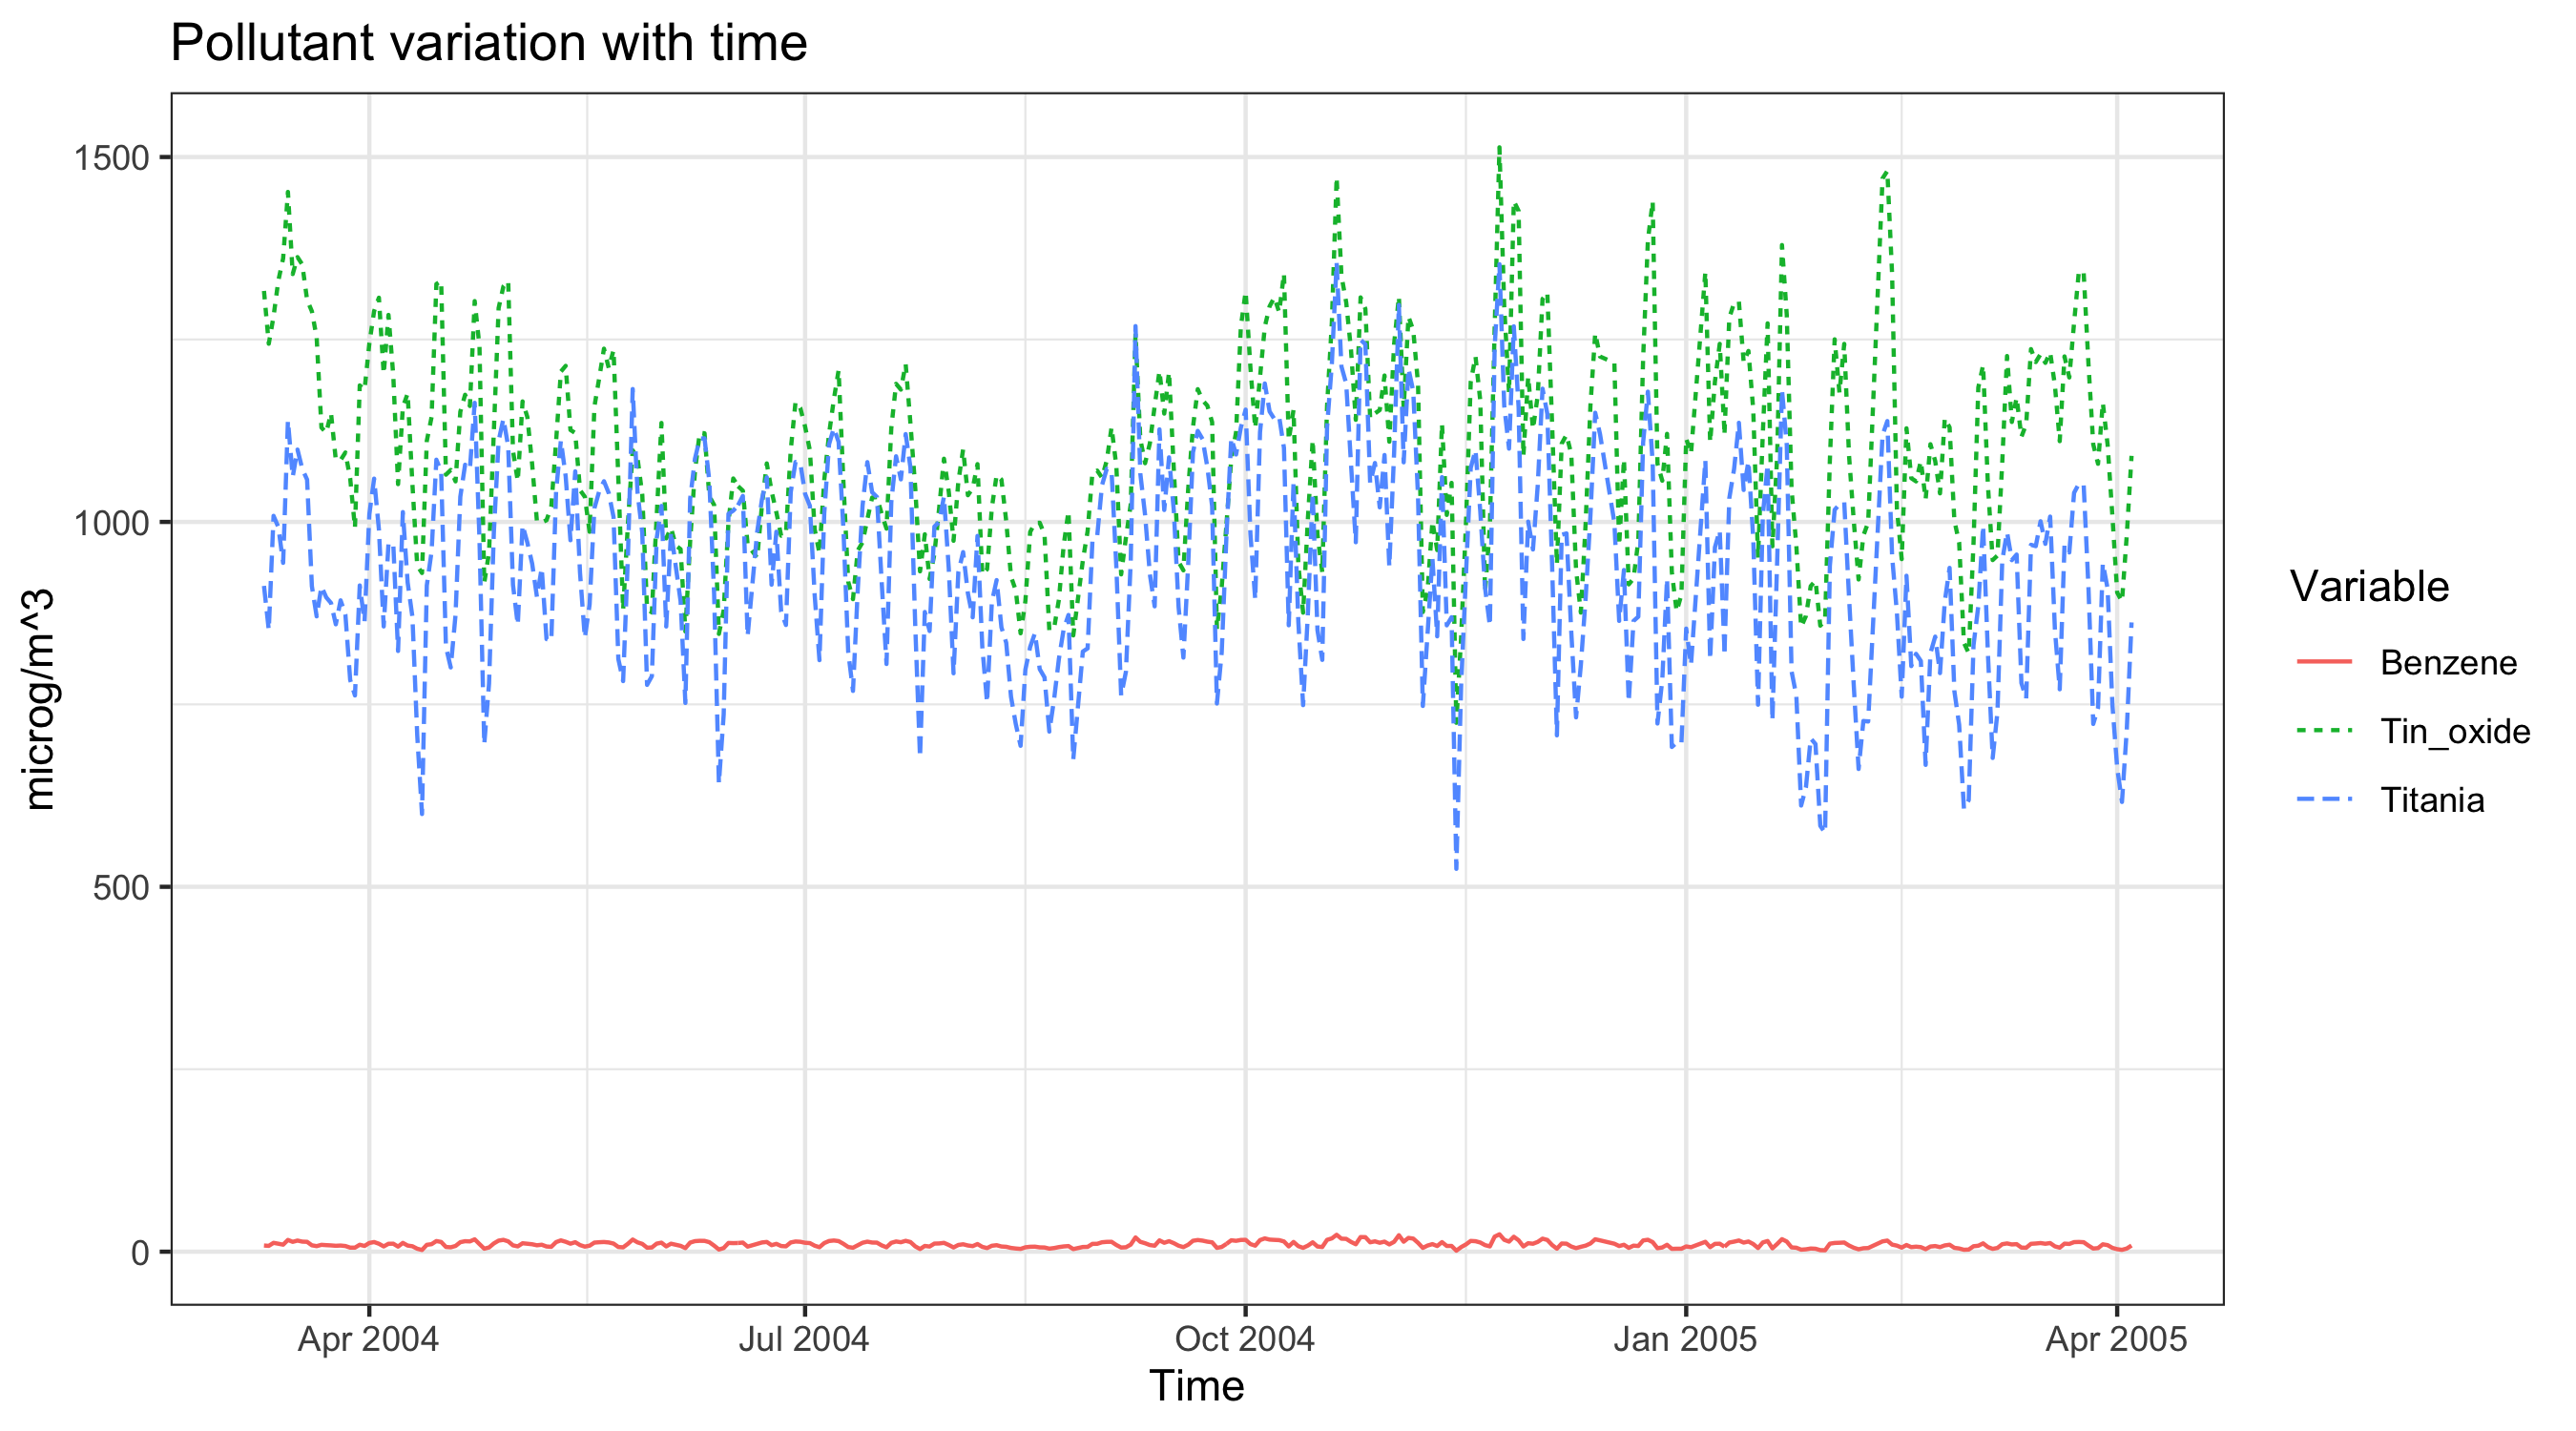
\includegraphics{../Images/pollutantsvstime.png}

\hypertarget{graph-3-concentration-temperature-and-humidity-over-time}{%
\subsubsection{Graph 3: Concentration Temperature and Humidity over
Time}\label{graph-3-concentration-temperature-and-humidity-over-time}}

The plot below show the \textbf{daily} averaged values of temperature
and humidity for a year.

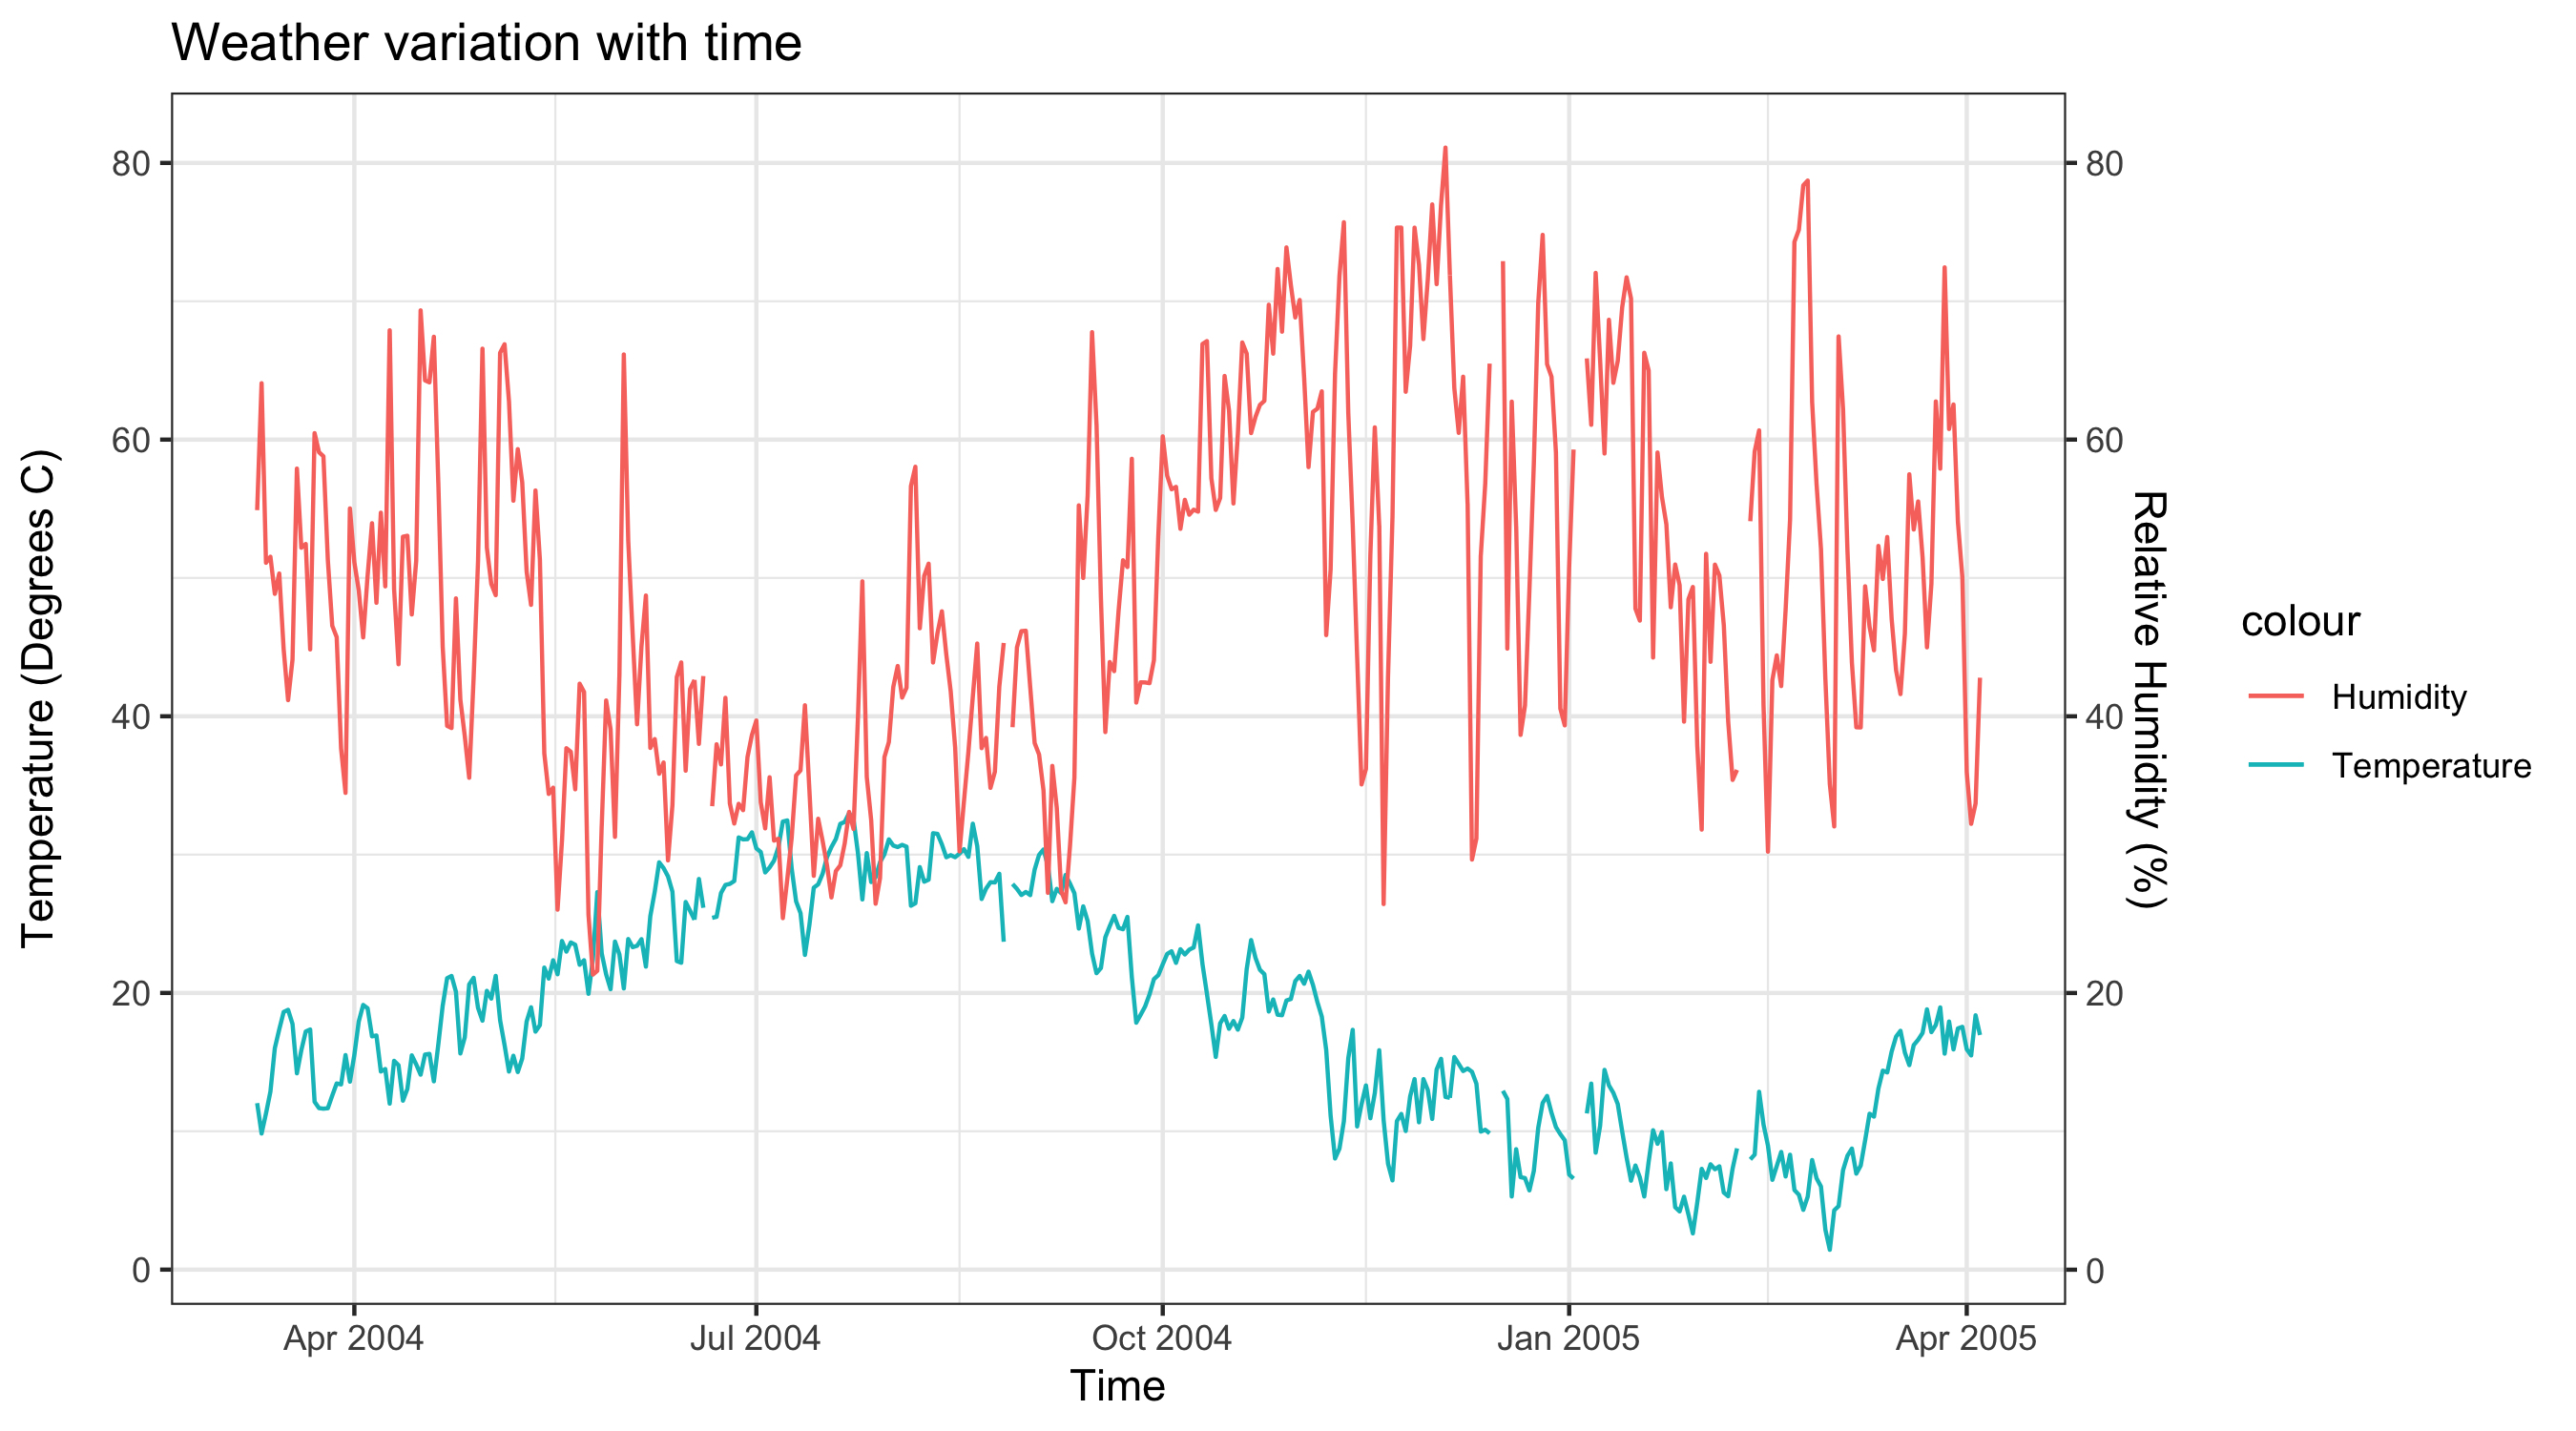
\includegraphics{../Images/weathervstime.png}

\hypertarget{graph-4-temperature-vs.benzene-concentration}{%
\subsubsection{Graph 4: Temperature vs.~Benzene
concentration}\label{graph-4-temperature-vs.benzene-concentration}}

The following graph shows the relationship of benzene to temperature
over the year in which data was recorded. The plot suggests there is
perhaps a slight relationship. Linear regression in future work will
help to clarify the relationships between weather and pollutant
concentrations.

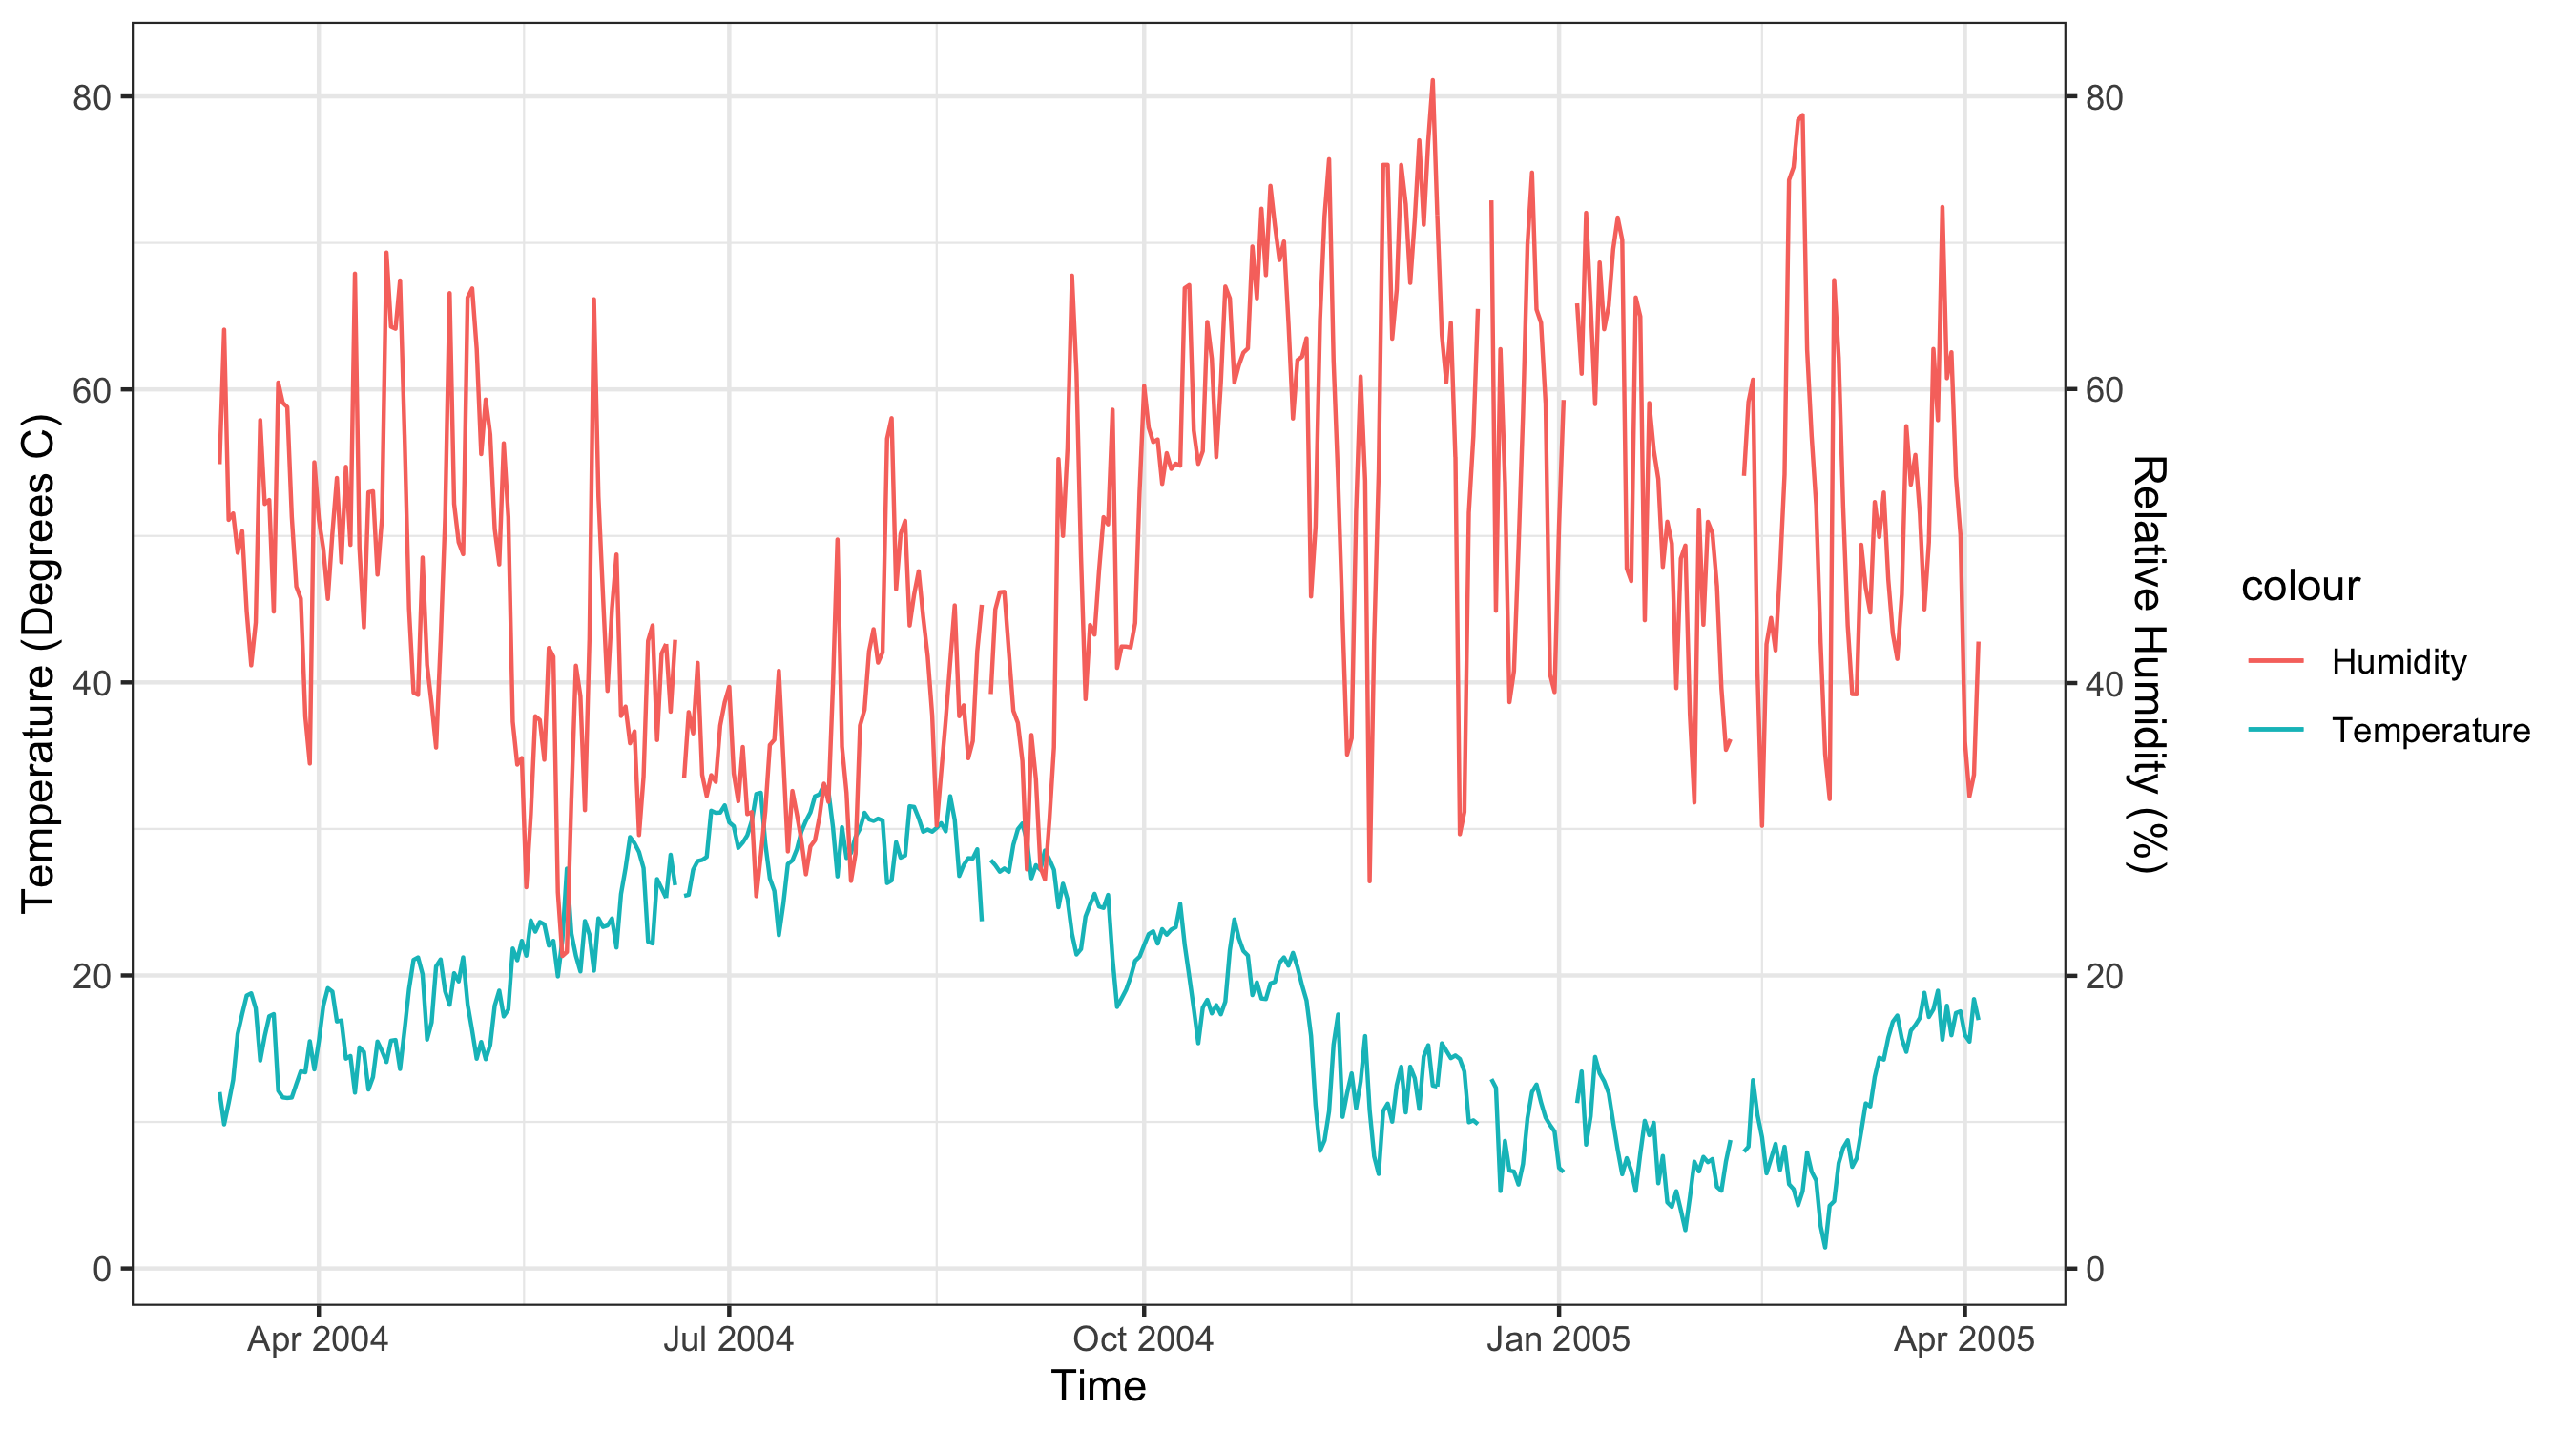
\includegraphics{../Images/tempvsbenzene.png}

\hypertarget{research-question}{%
\subsection{Research question}\label{research-question}}

In this analysis, we will attempt to determine the effects of
temperature and humidity on the concentration of air pollutants so our
research question is:

What is the affect of temperature and humidity on the concentration of
air pollutants, such as benzene, titania, and tin oxide?

\hypertarget{plan-of-action}{%
\subsection{Plan of action}\label{plan-of-action}}

With our research question, we are interested in the hourly averaged
concentrations of air pollutants, temperature and humidity. We will
ignore variables which have too many missing data to increase the
precision of this analysis. The air pollutants that we will focus on are
benzene, titania and tin oxide. After dealing with the missing data, we
will perform a linear regression analysis using OLS (ordinary least
square) method. Coefficients of relevant variables will be plotted with
confidence intervals.

\hypertarget{references}{%
\subsection{References}\label{references}}

S. De Vito, E. Massera, M. Piga, L. Martinotto, G. Di Francia, On field
calibration of an electronic nose for benzene estimation in an urban
pollution monitoring scenario, Sensors and Actuators B: Chemical, Volume
129, Issue 2, 22 February 2008, Pages 750-757, ISSN 0925-4005.

Matooane, M., John, J., Oosthuizen, R., and Binedell, M. 2004.
Vulnerability of South African communities to air pollution. In: 8th
World Congress on Environmental Health. Durban, South Africa: Document
Transformation Technologies.

Shea, K., Truckner, R., Weber, R., and Peden, D. 2008. Climate change
and allergic disease. Journal of Allergy and Clinical Immunology,
122(3): 443-453.

Younger, M., Morrow-Almeida, H., Vindigni, S., and Dannenberg, A. 2008.
The Built Environment, Climate Change, and Health Opportunities for
Co-Benefits. American Journal of Preventative Medicine, 35 (5): 517-526.


\end{document}
